% =========================================================================
% EvidenceTree — AAAI-format paper draft.
% NOTE: for actual AAAI submission, replace the preamble below with the
% official AAAI author kit (aaai2027.sty + aaai2027.bst) — this preamble
% only *mimics* the AAAI two-column camera-ready look so the draft compiles
% anywhere. Our own experimental numbers are intentionally left as "--"
% (training in progress); all baseline numbers are quoted from the cited
% papers (table sources given in each caption).
% =========================================================================
\documentclass[letterpaper,twocolumn,10pt]{article}

\usepackage[margin=0.75in,top=0.75in,bottom=1in,columnsep=0.25in]{geometry}
\usepackage{times}
\usepackage[T1]{fontenc}
\usepackage[utf8]{inputenc}
\usepackage{amsmath,amssymb,amsfonts,mathtools}
\usepackage{graphicx}
\usepackage{booktabs}
\usepackage{multirow}
\usepackage{makecell}
\usepackage{caption}
\usepackage{subcaption}
\usepackage{algorithm}
\usepackage{algpseudocode}
\usepackage{tikz}
\usetikzlibrary{arrows.meta,positioning,shapes.geometric,fit,backgrounds,calc}
\usepackage[numbers,sort&compress]{natbib} % swap for aaai27.bst author-year at submission
\usepackage{xcolor}
\usepackage[hidelinks]{hyperref}
\usepackage{enumitem}
\setlist{nosep,leftmargin=1.2em}

\captionsetup{font=small,labelfont=bf}
\newcommand{\ours}{EvidenceTree}
\newcommand{\dataset}{ETBench-Open}
\newcommand{\prm}{ET-PRM}
\newcommand{\NA}{--}          % our numbers: training in progress
\newcommand{\best}[1]{\textbf{#1}}

\title{\textbf{\ours: Grounded Process Reward Models for Monte Carlo Tree Search\\over Retrieval Actions in Multimodal Retrieval-Augmented Generation}}
\author{Anonymous submission}
\date{}

\begin{document}
\maketitle

% =========================================================================
\begin{abstract}
Multimodal retrieval-augmented generation (RAG) systems make a sequence of
retrieval decisions --- what to search, with which modality, and when to stop
--- yet these decisions are largely unsupervised: outcome-only rewards are
sparse and misassign credit, rule-based rewards are noisy, and existing
process reward models (PRMs) score \emph{reasoning steps under a fixed
context} rather than \emph{retrieval actions that modify the context}. We
present \ours{}, a multimodal RAG system that performs Monte Carlo Tree
Search (MCTS) directly over a typed retrieval action space
$\{\textsc{text\_search}, \textsc{image\_search}, \textsc{answer}\}$, guided
by a grounded, action-typed PRM trained specifically to evaluate
state-modifying retrieval actions. The PRM is supervised with a dual-source
step reward that fuses (i) a \emph{local grounding} signal --- the relevance
of each retrieved result to the question, measured in a single unified CLIP
embedding space so that text- and image-side evidence are comparable --- and
(ii) a \emph{tree-level outcome credit} --- the Monte Carlo success rate of
all rollouts passing through the node --- with an additional
\emph{answer-support gate} that prevents parametric lucky guesses from
receiving perfect labels. The PRM is trained generatively (rationale +
score) for dense supervision and queried score-only at inference for speed.
To train it we construct \dataset{}, a step-level annotated dataset of
retrieval trajectories built entirely on benchmark-provided corpora
(InfoSeek, ScienceQA, GQA) with a five-rule rationale quality-control
protocol that provably excludes ground-truth leakage. We report the
experimental protocol, baselines, and ablation design on InfoSeek,
ScienceQA, and GQA; our own results are withheld pending training
completion.
\end{abstract}

% =========================================================================
\section{Introduction}

Knowledge-intensive multimodal questions --- ``When did \emph{this} building
officially open?'', asked of a photograph --- cannot be answered from model
parameters alone: they require retrieving external evidence, often across
modalities \cite{chen2023infoseek,hu2023oven}. Retrieval-augmented
generation (RAG) has therefore become the dominant paradigm for
knowledge-based visual question answering (KB-VQA)
\cite{caffagni2024wikillava,yan2024echosight,lin2024preflmr}. However, the
\emph{retrieval decisions} of current systems are essentially unsupervised.
Fixed retrieve-then-generate pipelines apply the same recipe to every
question \cite{cocchi2025reflectiva}; reinforcement-learned search agents
receive only outcome-level rewards, which are sparse, misassign credit
across steps, and are known to induce process hallucination
\cite{wu2025mmsearchr1,wang2025vragrl}; and imitation-learned decision
agents \cite{chen2026learningtosearch} clone corrected search paths without
ever learning to \emph{evaluate} a retrieval action --- so a single bad
retrieval, once taken, silently corrupts everything downstream. Indeed,
\citet{chen2026learningtosearch} report that when retrieval goes wrong,
88.6\% of their agent's answers are wrong as well: linear agents cannot
recover from a bad search.

Process reward models (PRMs) offer the missing supervision signal: they
score intermediate steps rather than final outcomes
\cite{lightman2023verify,wang2024mathshepherd}. But existing PRMs ---
including multimodal ones \cite{visualprm2025} and grounded ones
\cite{groundedprm2025} --- evaluate \emph{reasoning steps under a fixed
state}: the image and context are given once and never change. This
assumption fails structurally in RAG, where every retrieval action
\emph{modifies} the state by appending evidence, where a step's quality
depends on what the retrieval actually returned, and where the system must
plan across modalities (search with text, or search with the image?). No
existing work simultaneously (A) evaluates the local quality of retrieval
actions with grounded signals, (B) supports backtracking when retrieval
fails, and (C) plans across retrieval modalities.

\ours{} fills this gap with three tightly coupled contributions:

\begin{itemize}
\item \textbf{An action-typed, grounded PRM for retrieval actions
(\prm{}).} The PRM scores candidate retrieval actions conditioned on the
question, the image, and the accumulated evidence bundle. Its training
labels fuse a graded \emph{local grounding} signal --- computed in one
unified CLIP space so text- and image-side results are on a comparable
scale --- with a \emph{tree-level outcome credit} that estimates each
node's true success potential by Monte Carlo, and an \emph{answer-support
gate} that blocks ``correct but evidence-free'' answers from receiving
perfect labels. The PRM is trained \emph{generatively} (rationale + score)
for dense supervision and anti-reward-hacking, and queried
\emph{score-only} at inference.
\item \textbf{Retrieval-action MCTS.} We build the search tree directly
over retrieval actions: nodes are partial contexts $(q, I, \mathcal{E})$,
edges are typed retrieval actions, and selection follows standard UCB1
with the PRM's value as the sole quality signal. Because the tree branches
over \emph{actions}, the system natively supports backtracking out of
failed retrieval branches --- the failure mode that linear agents cannot
escape --- and cross-modal planning arises from the PRM's learned
preference for image-based entity disambiguation followed by text-based
attribute lookup.
\item \textbf{\dataset{}.} A step-level annotated dataset of multimodal
retrieval trajectories (target 50--80K trajectories, $\sim$300K step
labels) constructed entirely on benchmark-provided corpora --- no live web
APIs, hence fully reproducible --- with a five-rule rationale
quality-control protocol that excludes ground-truth leakage by
construction. To our knowledge no existing dataset provides step-level
supervision for \emph{multimodal retrieval actions}: RAG-ProGuide
\cite{zhang2025reasonrag} is text-only, and DeepMMSearchVQA
\cite{deepmmsearch2025} provides trajectories without step-level labels.
\end{itemize}

We position \ours{} against the closest prior systems in
Section~\ref{sec:related}, detail the method in
Section~\ref{sec:method}, describe the dataset construction protocol in
Section~\ref{sec:dataset}, and lay out the complete experimental design ---
benchmarks, baselines with their published numbers, metrics, and ablations
--- in Section~\ref{sec:experiments}. Our own numbers are deliberately
withheld (marked ``\NA'') pending completion of PRM training; every
baseline number in our tables is quoted from the original publication
cited in the caption.

% -------------------------------------------------------------------------
\begin{figure*}[t]
\centering
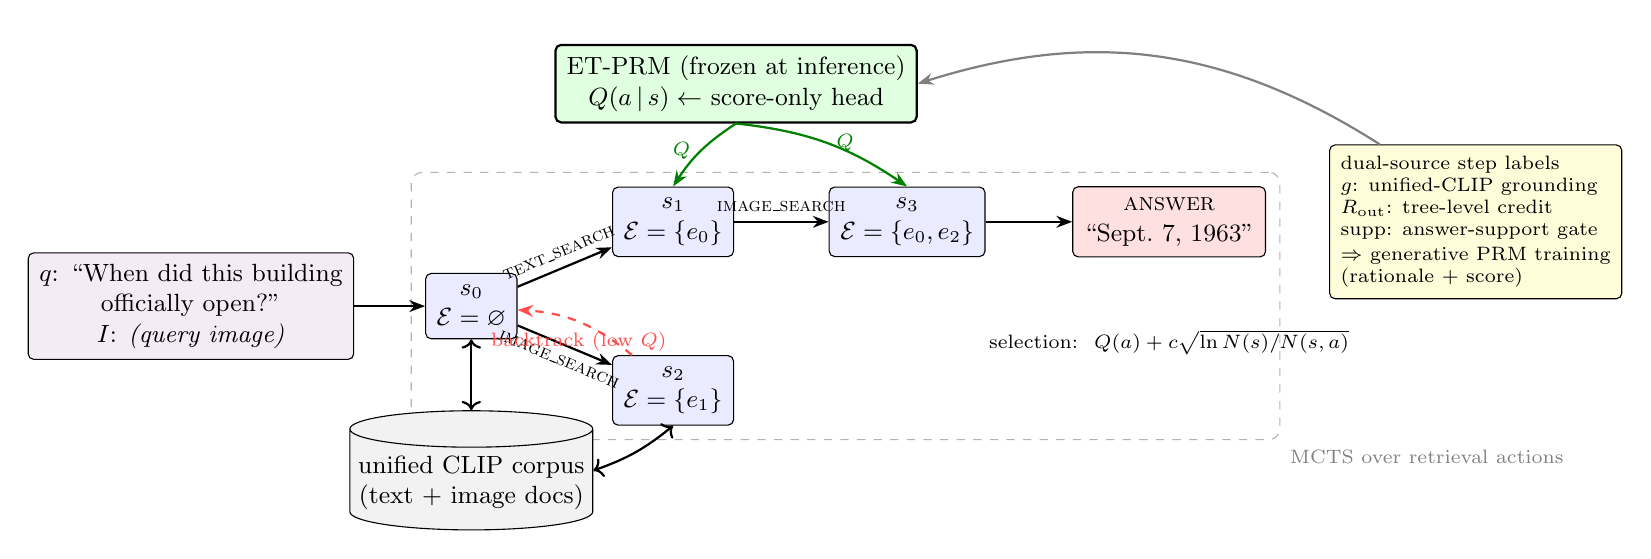
\begin{tikzpicture}[
  font=\small,
  node distance=4mm and 7mm,
  box/.style={draw,rounded corners=2pt,align=center,inner sep=4pt,minimum height=7mm},
  state/.style={box,fill=blue!8},
  act/.style={box,fill=orange!15},
  prmbox/.style={box,fill=green!12,thick},
  corpus/.style={cylinder,shape border rotate=90,draw,aspect=0.15,align=center,
                 inner sep=3pt,fill=gray!10,minimum height=11mm},
  arr/.style={-{Stealth[length=2mm]},thick},
]
% ----- left: query
\node[box,fill=violet!8] (query) {$q$: ``When did this building\\officially open?''\\$I$: \emph{(query image)}};
% ----- tree
\node[state,right=9mm of query] (root) {$s_0$\\$\mathcal{E}=\varnothing$};
\node[state,above right=2mm and 12mm of root] (s1) {$s_1$\\$\mathcal{E}=\{e_0\}$};
\node[state,below right=2mm and 12mm of root] (s2) {$s_2$\\$\mathcal{E}=\{e_1\}$};
\node[state,right=12mm of s1] (s3) {$s_3$\\$\mathcal{E}=\{e_0,e_2\}$};
\node[act,right=11mm of s3,fill=red!12] (ans) {\textsc{answer}\\``Sept.\ 7, 1963''};
\draw[arr] (query) -- (root);
\draw[arr] (root) -- node[above,sloped,font=\scriptsize]{\textsc{text\_search}} (s1);
\draw[arr] (root) -- node[below,sloped,font=\scriptsize]{\textsc{image\_search}} (s2);
\draw[arr] (s1) -- node[above,sloped,font=\scriptsize]{\textsc{image\_search}} (s3);
\draw[arr] (s3) -- (ans);
\draw[arr,dashed,red!70] (s2) to[bend right=18] node[below,font=\scriptsize,red!70]{backtrack (low $Q$)} (root);
% ----- corpus
\node[corpus,below=9mm of root] (corp) {unified CLIP corpus\\(text + image docs)};
\draw[arr,<->] (root) -- (corp);
\draw[arr,<->] (s2.south) to[bend left=10] (corp);
% ----- PRM
\node[prmbox,above=8mm of s1,xshift=8mm] (prm) {\prm{} (frozen at inference)\\$Q(a\,|\,s)\leftarrow$ score-only head};
\draw[arr,green!50!black] (prm.south) to[bend right=12] node[left,font=\scriptsize]{$Q$} (s1.north);
\draw[arr,green!50!black] (prm.south) to[bend left=14] node[right,font=\scriptsize]{$Q$} (s3.north);
% ----- UCB label
\node[below=8mm of ans,font=\scriptsize,align=center]
  {selection: $\;Q(a) + c\sqrt{\ln N(s)/N(s,a)}$};
% ----- training side
\begin{scope}[on background layer]
\node[fit=(root)(s1)(s2)(s3)(ans),draw=gray!60,dashed,rounded corners,inner sep=5pt,
      label={[gray,font=\scriptsize]south east:MCTS over retrieval actions}] {};
\end{scope}
\node[box,fill=yellow!15,right=8mm of ans,align=left,font=\scriptsize] (label)
  {dual-source step labels\\
   $g$: unified-CLIP grounding\\
   $R_\mathrm{out}$: tree-level credit\\
   $\mathrm{supp}$: answer-support gate\\[1pt]
   $\Rightarrow$ generative PRM training\\(rationale + score)};
\draw[arr,gray] (label) to[bend right=25] (prm.east);
\end{tikzpicture}
\caption{\textbf{\ours{} overview.} The search tree is built over
\emph{typed retrieval actions}; each edge executes a retrieval against the
benchmark-provided corpus (indexed in one unified CLIP space) and appends
the results to the evidence bundle $\mathcal{E}$. A grounded, action-typed
PRM provides the exploitation term $Q$ of UCB1 selection; low-$Q$ branches
are abandoned (backtracking). Training labels (right) fuse local grounding,
tree-level Monte Carlo outcome credit, and an answer-support gate, and the
PRM is trained generatively on \dataset{}.}
\label{fig:overview}
\end{figure*}

% =========================================================================
\section{Related Work}
\label{sec:related}

\paragraph{Tree search for multimodal RAG.}
RCTS \cite{rcts2025} performs MCTS over \emph{sets of retrieved
examples} to re-rank in-context demonstrations: the search happens after
retrieval, over a flat list of already-retrieved pairs, with rule-based
answer-matching rewards. AR-MCTS \cite{dong2025armcts} searches in
\emph{reasoning space}, using retrieval only to diversify expansion, and
trains a PRM over reasoning steps. \ours{} differs from both in \emph{where
the tree lives}: our nodes are partial retrieval contexts and our edges are
retrieval actions, so the search governs the retrieval process itself
rather than its aftermath. In text-only RAG, ReasonRAG
\cite{zhang2025reasonrag} builds process-supervised preference data via
MCTS over an agentic action space, and TreePS-RAG \cite{treeps2026}
estimates step utility from descendant outcomes; neither is multimodal,
neither trains a grounded PRM, and neither searches at inference time with
a learned action-value model.

\paragraph{Process reward models.}
PRMs originated in mathematical reasoning
\cite{lightman2023verify,wang2024mathshepherd}. VisualPRM
\cite{visualprm2025} extends process supervision to multimodal reasoning
but scores steps under a \emph{fixed} image context. GroundedPRM
\cite{groundedprm2025} verifies each reasoning step with external tools and
fuses tool-based local signals with MCTS-derived outcome signals into
rationale-enhanced generative supervision --- for mathematical reasoning.
We adopt its dual-source philosophy but transplant it to a setting it
explicitly does not cover: \emph{state-modifying} retrieval actions, where
the object being verified is what an action \emph{returned} rather than a
self-contained reasoning statement, where grounding must span modalities in
a single comparable space, and where credit must be assigned over a tree of
alternative retrievals. Step-level rewards for \emph{search} agents have
recently appeared in text-only settings
\cite{hipragr2025,ppr2026,decexrag2025}; generative PRMs for web agents
\cite{webarbiter2026} score browser actions. None combine multimodal
grounding, tree-level credit, and a learned generative PRM for retrieval
actions.

\paragraph{Agentic multimodal search.}
MMSearch-R1 \cite{wu2025mmsearchr1} trains an LMM with outcome-only GRPO to
invoke image and text search on demand; DeepMMSearch-R1
\cite{deepmmsearch2025} extends this with query-image cropping and a
dedicated VQA dataset; VRAG-RL \cite{wang2025vragrl} adds visual perception
actions. Closest to our setting, Learning-to-Search (DBAgent)
\cite{chen2026learningtosearch} reformulates KB-VQA as a four-action
decision process (\textsc{answer}/\textsc{image\_search}/%
\textsc{text\_search}/\textsc{caption}) over a curated Wikipedia corpus and
reaches state-of-the-art InfoSeek accuracy via supervised fine-tuning on
rule-constructed trajectories. All of these are \emph{linear} policies
learned by imitation or outcome-only RL: they neither estimate step values
nor backtrack. \ours{} is complementary --- it learns to \emph{evaluate}
retrieval actions and to \emph{plan} over them, keeping the policy
training-free; DBAgent's own analysis (29.6\% of its samples have correct
retrieval but wrong answers, and 88.6\% of wrong retrievals end in wrong
answers) is direct evidence for the value of step-level evaluation with
backtracking.

\paragraph{Step-level datasets.}
VisualPRM400K \cite{visualprm2025} contains almost exclusively mathematical
reasoning steps; RAG-ProGuide \cite{zhang2025reasonrag} provides 13K
process preference pairs for text-only RAG; DeepMMSearchVQA
\cite{deepmmsearch2025} provides multimodal search trajectories without
step labels. \dataset{} is, to our knowledge, the first step-level
annotated dataset of \emph{multimodal retrieval actions}, roughly an order
of magnitude larger than RAG-ProGuide at target scale.

% =========================================================================
\section{Method}
\label{sec:method}

\subsection{Problem Formulation}
\label{sec:formulation}

Given a question $q$ and an optional image $I$, the system interacts with a
fixed, benchmark-provided corpus $\mathcal{C}$ over multiple steps. The
state after $t$ steps is the partial retrieval context
\begin{equation}
s_t \;\triangleq\; \big(q,\; I,\; \mathcal{E}_t\big), \qquad
\mathcal{E}_t = \{e_1, \dots, e_{m_t}\},
\label{eq:state}
\end{equation}
where $\mathcal{E}_t$ is the \emph{evidence bundle} accumulated so far. At
each step the system selects an action $a_t \in \mathcal{A}$; retrieval
actions modify the state by appending their results,
$s_{t+1} = (q, I, \mathcal{E}_t \cup \mathrm{obs}(a_t))$, and the terminal
action emits an answer. A complete trajectory is
$\tau = (s_0, a_0, s_1, \dots, a_T)$ with $a_T = \textsc{answer}(y)$. The
goal is to choose the sequence of retrieval actions that maximizes the
probability that $y$ matches the gold answer $y^{*}$, under a fixed rollout
budget. Unlike reasoning-step search
\cite{dong2025armcts,visualprm2025}, every non-terminal action here is
\emph{state-modifying} and \emph{irreversible within its branch}: evidence,
once retrieved, conditions all subsequent decisions on that path. Tree
search provides the escape hatch --- a branch poisoned by a bad retrieval
can be abandoned rather than conditioned on.

\subsection{Retrieval Action Space}
\label{sec:actions}

We type actions by the \emph{modality of the retrieval query}, not of the
result:
\begin{equation}
\mathcal{A} = \{\, \textsc{text\_search}(x),\;
                   \textsc{image\_search}(I),\;
                   \textsc{answer}(y) \,\}.
\label{eq:actions}
\end{equation}
Both search actions query the \emph{same} unified index: every corpus
document --- text chunk or image --- is embedded with one CLIP model
\cite{radford2021clip}, so a text query or an image query retrieves
whichever side of the corpus is most similar. This yields the key
multimodal capability: for entity questions where the entity is not named
in $q$ (``this bird'', ``this building''), \textsc{image\_search} matches
the query image against the corpus to \emph{disambiguate the entity}, after
which \textsc{text\_search} retrieves the asked attribute using the
evidence-established entity name. We deliberately do not type actions by
result modality (a $2{\times}2$ split dilutes the visit counts of each
branch under small rollout budgets, and the retriever already decides
result modality by similarity), do not include compound parallel-search
actions (tree expansion already provides multi-candidate exploration, and
multi-source fusion is expressible as a serial trajectory), and do not
include state-invariant actions such as captioning (an edge that does not
change the observable state would receive no grounding signal and dilute
tree-level credit; captioning is folded into the policy prompt instead).
Appendix~\ref{app:actions} details these choices.

\subsection{Dual-Source Step Reward}
\label{sec:reward}

Each step of a trajectory receives a graded label in $[0,1]$ fusing two
complementary signals.

\paragraph{Local grounding.}
Grounding measures \emph{how relevant the results retrieved by this step
are to the question} --- deliberately scoring the result side rather than
the query side, since the query image of \textsc{image\_search} is fixed by
the state and carries no signal about whether the step helped. All results
are scored in one CLIP space against the same anchor:
\begin{equation}
g(a_t, s_t) \;=\; \max_{r \,\in\, \mathrm{obs}(a_t)}
  \phi_{m(r)}\!\Big( \cos\big( \mathrm{E}_\mathrm{T}(q),\,
  \mathrm{E}_{m(r)}(r) \big) \Big),
\label{eq:grounding}
\end{equation}
where $\mathrm{E}_\mathrm{T}$ and $\mathrm{E}_\mathrm{I}$ are the CLIP text
and image towers, $m(r)$ is the modality of result $r$, and $\phi_m$ is a
per-modality-pair linear calibration band mapping the raw cosine onto a
common $[0,1]$ relevance scale (same-modality cosines run systematically
higher than cross-modal ones). Empty results give $g = 0$. Using a
\emph{single} model for both sides is essential: two different encoders
would put text- and image-side evidence on different cosine scales, and the
PRM would mistake the scale gap for a quality gap, systematically biasing
action selection. All grounding scores are graded, not binary --- retrieval
quality in open corpora is not a 0/1 property (cf.\ the binary verification
of \citealt{groundedprm2025}).

\paragraph{Tree-level outcome credit.}
Outcome credit estimates each node's true success potential. For a node
reached by the action prefix $\pi_t = (a_0, \dots, a_t)$ within one
question's search tree, let $\mathcal{T}(\pi_t)$ denote all complete
rollouts passing through it. Then
\begin{equation}
R_\mathrm{out}(s_t, a_t) \;=\;
\frac{1}{|\mathcal{T}(\pi_t)|} \sum_{\tau \in \mathcal{T}(\pi_t)}
\mathbb{1}\!\left[ y(\tau) \approx y^{*} \right],
\label{eq:credit}
\end{equation}
a Monte Carlo estimate of the success rate \emph{from this node onward}.
This is crucially different from uniformly smearing a trajectory's final
reward over its steps --- uniform credit rewards the bad steps of lucky
trajectories and punishes the good steps of unlucky ones, whereas
Eq.~\eqref{eq:credit} lets two children of the same node receive sharply
different labels (cf.\ shortest-path estimation in
\citealt{zhang2025reasonrag}; descendant-outcome utilities in
\citealt{treeps2026}). Answer matching $\mathbb{1}[\cdot \approx y^{*}]$
follows each benchmark's official protocol (relaxed numeric-range matching
for InfoSeek VALUE questions; Appendix~\ref{app:dataset}).

\paragraph{Fusion and the answer-support gate.}
Non-terminal steps fuse the two sources linearly:
\begin{equation}
R(s_t, a_t) \;=\; \alpha\, g(a_t, s_t) + (1-\alpha)\, R_\mathrm{out}(s_t, a_t),
\label{eq:fusion}
\end{equation}
with $\alpha = 0.5$ by default (sensitivity in
Section~\ref{sec:ablations}). Terminal \textsc{answer} steps have no
retrieval result to ground, and labeling them by outcome alone creates a
subtle poison: a \emph{parametric lucky guess} --- an answer that happens
to be correct although nothing in the evidence supports it --- would
receive a perfect label, teaching the PRM that evidence-free answering is
optimal. We therefore gate the outcome by an \emph{answer-support} verdict
$\mathrm{supp}(y, \mathcal{E}_T) \in [0,1]$, judged by an LLM over the
accumulated evidence (four-way rubric:
\textsc{supported}/\textsc{partial}/\textsc{unsupported} $\mapsto$
$1/0.5/0$, plus \textsc{not\_required} $\mapsto$ no gating for questions
answerable from the question and image alone by perception or logic ---
entailment-gating those would systematically punish correct reasoning
answers; Appendix~\ref{app:support}):
\begin{equation}
R_\mathrm{ans}(s_T) \;=\; R_\mathrm{out}(s_T, a_T)\cdot
\big( \gamma + (1-\gamma)\,\mathrm{supp}(y, \mathcal{E}_T) \big),
\label{eq:support}
\end{equation}
with floor $\gamma = 0.3$. The multiplicative form keeps wrong answers at
zero regardless of spurious support; the floor preserves the ordering
\emph{wrong} $<$ \emph{correct-but-unsupported} ($\approx\gamma$) $<$
\emph{correct-and-supported} ($\approx 1$) and buffers verifier noise.
Correct-but-unsupported answers are additionally flagged --- not discarded
--- as ready-made rejected sides for preference training
(Section~\ref{sec:training}).

\subsection{\prm{}: Architecture and Training}
\label{sec:training}

\paragraph{Architecture.}
\prm{} is initialized from VisualPRM-8B \cite{visualprm2025} (itself built
on InternVL2.5-8B \cite{chen2024internvl}), inheriting multimodal
inductive biases, with an action-conditional value readout. The input
serializes the state and the candidate action:
question and image, the evidence bundle, and the candidate action's type
and parameters; the output is a rationale followed by a score token.

\paragraph{Generative training, score-only inference.}
Following the generative reward modeling paradigm
\cite{zhang2024generative,ankner2024critique}, \prm{} is trained to emit a
natural-language rationale \emph{and} a score. This is a deliberate choice
with three payoffs at our data scale: each sample supervises dozens of
tokens rather than one scalar (sample efficiency); the model must
articulate \emph{why} an action deserves its score, exposing spurious
shortcuts (anti-reward-hacking); and failed training runs can be diagnosed
by reading rationales. At inference the rationale is skipped entirely ---
only the score-token logit is read --- so MCTS pays no generation latency.

\paragraph{Three training stages.}
\emph{(1) SFT}: next-token prediction on \dataset{} (state, action,
rationale, score). \emph{(2) Action-typed preference optimization}: DPO
\cite{rafailov2023dpo} on same-state contrastive pairs mined from the
search trees --- (successful sibling action, failed action),
(\textsc{text\_search}, \textsc{image\_search}) under the same state, and
(supported answer, unsupported-correct answer), the latter using the
flagged samples of Eq.~\eqref{eq:support}. Pair construction exploits the
same node keys as Eq.~\eqref{eq:credit}, so the contrast dimension is
``same state, different action'' --- matching the decision the searcher
actually faces --- rather than the step-position contrasts used for
reasoning PRMs. \emph{(3) Calibration}: temperature/Platt scaling of the
score logit on held-out data, so that $Q$ values entering UCB1 have
probabilistic meaning.

\subsection{PRM-Guided MCTS over Retrieval Actions}
\label{sec:search}

Search follows the four canonical MCTS phases with the PRM as the value
oracle. \emph{Selection} descends by UCB1
\cite{auer2002ucb,kocsis2006uct}:
\begin{equation}
a^{\dagger} = \arg\max_{a}\;
Q(a \mid s) \;+\; c\, \sqrt{ \frac{\ln N(s)}{N(s, a)} },
\label{eq:ucb}
\end{equation}
where $Q$ is the running mean of backed-up rewards seeded by the PRM prior
for unvisited edges, and $c = 1.0$ by default. We use \emph{no} additional
novelty or modality-coverage bonus: the PRM's $Q$ is the sole quality
signal, and hard-coded exploration preferences would both dilute it and add
tuning burden (Appendix~\ref{app:actions}). \emph{Expansion} asks a
training-free policy VLM to propose candidate actions (with
anti-fabrication and retrieval-chain constraints in the prompt;
Appendix~\ref{app:prompts}), executes them against the local index, and
keeps the top-$k$ by PRM prior. \emph{Simulation} rolls out greedily to a
forced answer at depth $d_{\max}$. \emph{Backup} propagates the trajectory
reward to the root. Search stops early when the best root path exceeds a
quality threshold, or when the rollout budget $P$ is exhausted (defaults:
$P{=}10$, $d_{\max}{=}3$, $k{=}3$). Algorithm~\ref{alg:search} summarizes
the loop.

\begin{algorithm}[t]
\caption{\ours{} inference}
\label{alg:search}
\begin{algorithmic}[1]
\Require question $q$, image $I$, corpus index, budget $P$, depth $d_{\max}$
\State $\mathrm{root} \gets (q, I, \varnothing)$
\For{$t = 1 \dots P$}
  \State $s \gets$ \textsc{Select}(root) by Eq.~\eqref{eq:ucb}
  \State $\mathcal{A}_c \gets$ policy proposals at $s$; execute retrievals
  \State keep top-$k$ children of $s$ by PRM prior $Q(a \mid s)$
  \State $\tau \gets$ \textsc{Simulate} greedily to \textsc{answer} or $d_{\max}$
  \State \textsc{Backup}$(\tau, R_\mathrm{PRM}(\tau))$
  \If{$\max_{\tau} R_\mathrm{PRM}(\tau) > \tau_{\mathrm{stop}}$} \textbf{break}
  \EndIf
\EndFor
\State \Return answer of the highest-value root path
\end{algorithmic}
\end{algorithm}

% =========================================================================
\section{The \dataset{} Dataset}
\label{sec:dataset}

\begin{figure}[t]
\centering
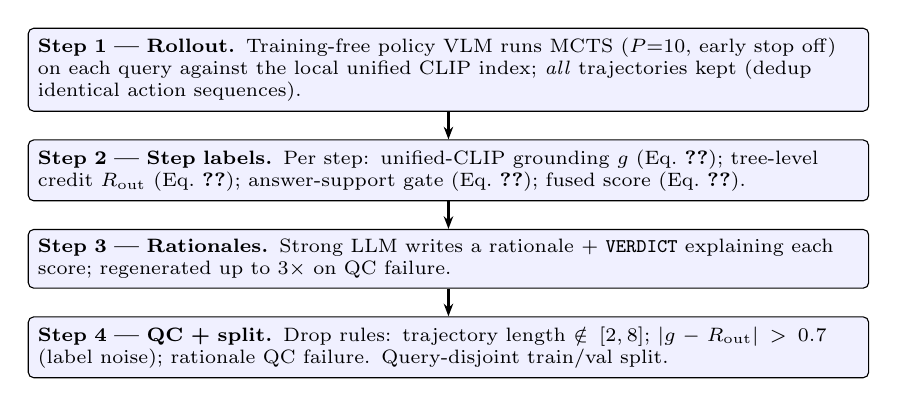
\begin{tikzpicture}[
  font=\scriptsize, node distance=3.5mm,
  stage/.style={draw,rounded corners=2pt,align=left,inner sep=3.5pt,
               fill=blue!6,text width=0.86\linewidth},
  arr/.style={-{Stealth[length=1.6mm]},thick},
]
\node[stage] (s1) {\textbf{Step 1 — Rollout.} Training-free policy VLM runs
MCTS ($P{=}10$, early stop off) on each query against the local unified
CLIP index; \emph{all} trajectories kept (dedup identical action
sequences).};
\node[stage,below=of s1] (s2) {\textbf{Step 2 — Step labels.} Per step:
unified-CLIP grounding $g$ (Eq.~\ref{eq:grounding}); tree-level credit
$R_\mathrm{out}$ (Eq.~\ref{eq:credit}); answer-support gate
(Eq.~\ref{eq:support}); fused score (Eq.~\ref{eq:fusion}).};
\node[stage,below=of s2] (s3) {\textbf{Step 3 — Rationales.} Strong LLM
writes a rationale + \texttt{VERDICT} explaining each score; regenerated
up to 3$\times$ on QC failure.};
\node[stage,below=of s3] (s4) {\textbf{Step 4 — QC + split.} Drop rules:
trajectory length $\notin[2,8]$; $|g - R_\mathrm{out}| > 0.7$ (label
noise); rationale QC failure. Query-disjoint train/val split.};
\draw[arr] (s1) -- (s2); \draw[arr] (s2) -- (s3); \draw[arr] (s3) -- (s4);
\end{tikzpicture}
\caption{\textbf{\dataset{} construction pipeline.} Retrieval is fully
offline (local indices over benchmark-provided corpora); the only external
API is the one-time rationale/support judging, whose outputs ship with the
dataset --- the construction is reproducible end to end.}
\label{fig:pipeline}
\end{figure}

\dataset{} is built by the four-step pipeline of
Figure~\ref{fig:pipeline}, entirely on corpora that ship with the
benchmarks: a Wikipedia entity corpus for InfoSeek (chunked full pages of
the 1{,}794 validation entities), the lecture/context corpus for
ScienceQA, and scene-graph-derived textual documents paired with images
for GQA. This design has three consequences we consider essential for a
paper about \emph{decision quality}: reproducibility (no live-web drift),
causal cleanliness (performance differences cannot be explained by ``the
web changed''), and auditability (every evidence item in every label is a
corpus document with a stable identifier).

\paragraph{Rationale quality control.}
Generative PRM training is only as good as its rationales. Each rationale
must (a) cite at least one evidence identifier visible in the sample, (b)
name the action type, (c) be 30--150 tokens, (d) contain \emph{no
ground-truth leakage} --- no evaluation phrasing, and no gold-answer string
that is absent from the sample's visible evidence, question, and action
input (quoting the answer \emph{from cited evidence} is legitimate;
knowing it without evidence is leakage --- rationales must argue
\emph{ex-ante}, as at inference the PRM has no oracle), and (e) end with a
\texttt{VERDICT} tag that must not contradict the numeric score
(preventing say-one-thing-score-another training pairs). Rules (d)/(e)
adapt the trajectory-realism constraints of
\citet{chen2026learningtosearch} from policy imitation to reward-model
supervision.

\paragraph{Scale and status.}
Target scale is 50--80K trajectories ($\sim$300K step labels) across the
three benchmarks. Construction statistics of a completed 100-query-per-%
benchmark pilot --- including the step-label and support-verdict
distributions that motivated the support gate --- are reported in
Appendix~\ref{app:pilot}. Full-scale construction and PRM training are in
progress; accordingly, all \ours{} result cells in
Section~\ref{sec:experiments} are marked ``\NA''.

% =========================================================================
\section{Experimental Design}
\label{sec:experiments}

\subsection{Setup}
\label{sec:setup}

\paragraph{Benchmarks and metrics.}
We evaluate on three benchmarks with complementary demands.
\textbf{InfoSeek} \cite{chen2023infoseek}: fine-grained entity knowledge
VQA over a Wikipedia corpus; validation split, official relaxed accuracy
(string questions: relaxed exact match over the gold set; numeric
questions: any predicted number inside the gold range), reported on
Unseen-Question / Unseen-Entity / All. \textbf{ScienceQA}
\cite{lu2022scienceqa}: multiple-choice science questions; test split
accuracy. \textbf{GQA} \cite{hudson2019gqa}: compositional VQA over real
images; test-dev balanced accuracy. ScienceQA and GQA are not
knowledge-seeking in the InfoSeek sense; we include them to probe two
specific behaviors --- whether the PRM learns \emph{when not to retrieve}
(ScienceQA reasoning questions) and whether image-query retrieval provides
clean perception evidence (GQA scene-graph corpus) --- and we analyze them
separately from the open-domain headline results.

\paragraph{Implementation.}
Policy: Qwen2.5-VL-7B-Instruct \cite{bai2025qwen25vl}, training-free
(prompt in Appendix~\ref{app:prompts}). Retrieval: BM25
\cite{robertson2009bm25} and dense CLIP indices (FAISS
\cite{johnson2019faiss}) built offline per benchmark corpus; text top-3,
image top-1 following \citet{chen2026learningtosearch}. PRM: VisualPRM-8B
fine-tuned with LoRA \cite{hu2022lora} through the three stages of
Section~\ref{sec:training}. Search: $P{=}10$, $d_{\max}{=}3$, $k{=}3$,
$c{=}1.0$, $\alpha{=}0.5$, $\gamma{=}0.3$. All results (once reported)
will be means over 3 seeds.

\subsection{Baselines}
\label{sec:baselines}

We compare against four families: (i) zero-shot MLLMs (no retrieval);
(ii) fixed-pipeline multimodal RAG; (iii) reflection- or process-enhanced
RAG; (iv) agentic / decision-based search including the strongest published
InfoSeek system, DBAgent \cite{chen2026learningtosearch}; plus
PRM-with-Best-of-$N$ controls (frozen VisualPRM-8B reranking $N$ sampled
trajectories) that isolate the contribution of tree search over
sample-and-rerank. Baseline numbers in
Tables~\ref{tab:infoseek}--\ref{tab:gqa} are quoted from the cited
publications; rows we will run ourselves under our corpus protocol are
marked accordingly.

% ---------------- Main tables (baselines quoted from cited papers)
\begin{table}[t]
\centering\small
\setlength{\tabcolsep}{3.5pt}
\begin{tabular}{@{}llccc@{}}
\toprule
Method & Backbone & Un-Q & Un-E & All \\
\midrule
\multicolumn{5}{@{}l}{\emph{Zero-shot MLLMs (no retrieval)}} \\
BLIP-2 \cite{li2023blip2} & Flan-T5-XXL & 12.7 & 12.3 & 12.5 \\
InstructBLIP \cite{dai2023instructblip} & Flan-T5-XXL & 8.9 & 7.4 & 8.1 \\
LLaVA-1.5 \cite{liu2024llava15} & Vicuna-7B & 9.6 & 9.4 & 9.5 \\
GPT-4V$^{\S}$ & -- & 15.0 & 14.3 & 14.6 \\
Qwen2.5-VL$^{\S}$ \cite{bai2025qwen25vl} & 7B & 22.8 & 24.1 & 23.7 \\
\midrule
\multicolumn{5}{@{}l}{\emph{Retrieval-augmented (fixed pipeline / reflective)}} \\
Wiki-LLaVA \cite{caffagni2024wikillava} & LLaVA-1.5-7B & 30.1 & 27.8 & 28.9 \\
PreFLMR \cite{lin2024preflmr} & RA-VQAv2 & -- & -- & 30.7 \\
EchoSight \cite{yan2024echosight} & LLaMA-3-8B & -- & -- & 31.3 \\
RoRA-VLM \cite{qi2024roravlm} & Vicuna-7B & 25.1 & 27.3 & -- \\
ReflectiVA \cite{cocchi2025reflectiva} & LLaMA-3.1-8B & 40.4 & 39.8 & 40.1 \\
Wiki-PRF \cite{hong2025wikiprf} & Qwen2.5-VL-7B & 43.3 & 42.7 & 42.8 \\
\midrule
\multicolumn{5}{@{}l}{\emph{Agentic / decision-based search}} \\
Wiki-R1 \cite{wikir12026} & Qwen2.5-VL-7B & \best{47.8} & -- & 44.1 \\
DBAgent \cite{chen2026learningtosearch} & Qwen2.5-VL-7B & 46.5 & \best{51.0} & \best{49.9} \\
\midrule
VisualPRM-8B + BoN$^\ddagger$ & Qwen2.5-VL-7B & \NA & \NA & \NA \\
\ours{} (ours) & Qwen2.5-VL-7B & \NA & \NA & \NA \\
\bottomrule
\end{tabular}
\caption{\textbf{InfoSeek} (validation, official relaxed accuracy).
Baseline numbers are quoted from the cited papers%
 (BLIP-2/InstructBLIP from the official evaluation kit of \citealt{chen2023infoseek}; Wiki-LLaVA and LLaVA-1.5 from \citealt{caffagni2024wikillava}, Table~2; EchoSight from \citealt{yan2024echosight}; PreFLMR from \citealt{lin2024preflmr}, Table~7, whose authors note a pre-release InfoSeek setup; RoRA-VLM from \citealt{qi2024roravlm}; ReflectiVA from \citealt{cocchi2025reflectiva}; Wiki-PRF from \citealt{hong2025wikiprf}; Wiki-R1 from \citealt{wikir12026}, unseen-entity split not reported; DBAgent (SFT on InfoSeek trajectories) from \citealt{chen2026learningtosearch}, Table~1. $\S$: zero-shot numbers as compiled in \citealt{chen2026learningtosearch}, Table~1.)
. $\ddagger$: control we run under the identical corpus protocol. ``\NA'':
training in progress.}
\label{tab:infoseek}
\end{table}

\begin{table}[t]
\centering\small
\setlength{\tabcolsep}{4pt}
\begin{tabular}{@{}llc@{}}
\toprule
Method & Backbone & Acc. \\
\midrule
Human \cite{lu2022scienceqa} & -- & 88.40 \\
MM-CoT \cite{zhang2023mmcot} & UnifiedQA-738M & 91.68 \\
LLaVA (fine-tuned) \cite{liu2023visualinstruction} & Vicuna-13B & 90.92 \\
Zero-shot$^{\dagger}$ & Qwen2-VL-7B & 80.33 \\
Zero-shot$^{\dagger}$ & InternVL2-8B & 93.00 \\
Vanilla RAG$^{\dagger}$ & Qwen2-VL-7B & 86.68 \\
RCTS \cite{rcts2025} & Qwen2-VL-7B & 91.44 \\
RCTS \cite{rcts2025} & InternVL2-8B & \best{94.20} \\
\midrule
VisualPRM-8B + BoN$^\ddagger$ & Qwen2.5-VL-7B & \NA \\
\ours{} (ours) & Qwen2.5-VL-7B & \NA \\
\bottomrule
\end{tabular}
\caption{\textbf{ScienceQA} (test accuracy). Baseline numbers quoted from
the cited papers%
 (MM-CoT from \citealt{zhang2023mmcot}; LLaVA from \citealt{liu2023visualinstruction}, Table~7; $\dagger$: as measured in the RCTS paper \citealt{rcts2025} under its evaluation protocol; RCTS from the same table. AR-MCTS \citealt{dong2025armcts} does not evaluate on ScienceQA; methods reporting only the IMG subset, e.g.\ LLaVA-1.5 at 66.8, are omitted for protocol consistency.)
.}
\label{tab:scienceqa}
\end{table}

\begin{table}[t]
\centering\small
\setlength{\tabcolsep}{4pt}
\begin{tabular}{@{}llc@{}}
\toprule
Method & Backbone & Acc. \\
\midrule
BLIP-2$^{\ast}$ \cite{li2023blip2} & Vicuna-13B & 41.0 \\
InstructBLIP \cite{dai2023instructblip} & Vicuna-7B & 49.2 \\
Qwen-VL-Chat \cite{bai2023qwenvl} & Qwen-7B & 57.5 \\
Qwen-VL \cite{bai2023qwenvl} & Qwen-7B & 59.3 \\
LLaVA-1.5 \cite{liu2024llava15} & Vicuna-7B & 62.0 \\
LLaVA-1.5 \cite{liu2024llava15} & Vicuna-13B & \best{63.3} \\
\midrule
\ours{} (ours) & Qwen2.5-VL-7B & \NA \\
\bottomrule
\end{tabular}
\caption{\textbf{GQA} (test-dev balanced accuracy). Baseline numbers quoted
from the cited papers%
 (Qwen-VL rows from \citealt{bai2023qwenvl}; LLaVA-1.5 and InstructBLIP from \citealt{liu2024llava15} and \citealt{dai2023instructblip}; $\ast$: zero-shot number as reported in \citealt{liu2024llava15}, Table~1. Existing multimodal RAG and tree-search systems do not report GQA; we include it to probe perception-evidence retrieval over a scene-graph corpus, not as an open-domain RAG battlefield.)
.}
\label{tab:gqa}
\end{table}

\subsection{Ablation Design}
\label{sec:ablations}

Table~\ref{tab:ablations} pre-registers the ablation grid. \textbf{A1}
tests whether both reward sources are necessary ($\alpha \in \{0, 0.2,
0.5, 0.8, 1\}$) and whether the support gate matters (Eq.~\ref{eq:support}
on/off). \textbf{A2} varies the exploration constant ($c \in \{0, 0.5, 1,
2\}$; $c{=}0$ is greedy PRM). \textbf{A3} accumulates the PRM training
stages (SFT / +DPO / +calibration) against the frozen VisualPRM-8B
zero-shot scorer. \textbf{A4} grows the action space
(\textsc{text\_search}-only $\rightarrow$ +\textsc{image\_search}).
\textbf{A5} varies the search budget ($d_{\max} \in \{2,3,5\}$, $P \in
\{4,10,20\}$) against Best-of-$N$ at matched PRM-call budgets --- the
decisive test that \emph{tree} search, not merely PRM reranking, carries
the gains. \textbf{A6} evaluates robustness under corpus poisoning
\cite{poisonedmrag2025}: 5--20 adversarial image--text pairs injected per
query; we measure the answer flip rate with and without PRM-guided
backtracking.

\begin{table}[t]
\centering\small
\setlength{\tabcolsep}{3pt}
\begin{tabular}{@{}llccc@{}}
\toprule
Ablation & Variant & InfoSeek & SQA & GQA \\
\midrule
\multirow{3}{*}{A1 reward}
 & local only ($\alpha{=}1$) & \NA & \NA & \NA \\
 & outcome only ($\alpha{=}0$) & \NA & \NA & \NA \\
 & no support gate & \NA & \NA & \NA \\
\midrule
\multirow{2}{*}{A2 search}
 & greedy ($c{=}0$) & \NA & \NA & \NA \\
 & $c \in \{0.5, 2.0\}$ & \NA & \NA & \NA \\
\midrule
\multirow{3}{*}{A3 PRM}
 & frozen VisualPRM & \NA & \NA & \NA \\
 & SFT only & \NA & \NA & \NA \\
 & SFT+DPO & \NA & \NA & \NA \\
\midrule
\multirow{2}{*}{A4 actions}
 & text-only & \NA & \NA & \NA \\
 & + image search & \NA & \NA & \NA \\
\midrule
\multirow{2}{*}{A5 budget}
 & BoN, matched calls & \NA & \NA & \NA \\
 & $P{=}4 / 20$ & \NA & \NA & \NA \\
\bottomrule
\end{tabular}
\caption{Pre-registered ablation grid (accuracy; ``\NA'' = training in
progress). A6 (poisoning robustness) reports answer flip rate and is
tabulated separately.}
\label{tab:ablations}
\end{table}

\subsection{Analysis Protocol}
Beyond headline accuracy we will report: (i) the retrieval-correctness
$\times$ answer-correctness contingency table, whose off-diagonal mass
motivates step-level evaluation (cf.\ 29.6\%/88.6\% in
\citealt{chen2026learningtosearch}); (ii) PRM score--outcome correlation
(Spearman/AUC) against the frozen VisualPRM-8B diagnostic baseline; (iii)
per-action-type PRM calibration curves; and (iv) corpus-scale robustness
(10K $\rightarrow$ 100K documents).

% =========================================================================
\section{Conclusion}
\ours{} moves grounded process supervision from fixed-state reasoning to
state-modifying retrieval actions: a PRM that evaluates what a retrieval
\emph{returned} (in one unified multimodal embedding space), credits each
node by the Monte Carlo success of the subtree behind it, refuses to reward
evidence-free lucky answers, and guides a standard UCB1 tree search that
can back out of poisoned branches. The accompanying \dataset{} provides the
first step-level supervision for multimodal retrieval actions, with a
leakage-proof rationale protocol. The experimental grid is fully specified;
results will populate the ``\NA'' cells upon training completion.

% =========================================================================
\bibliographystyle{plainnat} % swap for aaai27.bst at submission
\bibliography{references}

% =========================================================================
\clearpage
\appendix

\section{Action Space: Rejected Designs}
\label{app:actions}
\paragraph{Why not a $2{\times}2$ (query $\times$ result) action split.}
Under a rollout budget of $P{=}10$, four search actions halve per-branch
visit counts; result modality is better decided by the retriever's
similarity in the unified index; and grounding already scores by the
\emph{actual} modality of each returned result
(Eq.~\ref{eq:grounding}), so the action type need not carry it.
\paragraph{Why no \textsc{parallel\_search}.}
Tree expansion already explores multiple candidates (OR-semantics), and
AND-semantics (fuse evidence from two sources) is expressible serially ---
search $A$, then $B$; the bundle accumulates. A compound action would need
bespoke grounding (means over sub-actions), conflict with tree-level
credit, and dilute the budget.
\paragraph{Why no \textsc{caption} action.}
Captioning does not modify the observable state: an edge with an unchanged
state has no retrieval result to ground ($g$ undefined), creates
parent-child duplicates that dilute Eq.~\eqref{eq:credit}, and burns
budget. The policy VLM sees the image directly, so caption-style
verbalization is folded into the proposal prompt
(Appendix~\ref{app:prompts}); cf.\ the caption action of
\citet{chen2026learningtosearch}, which their inference likewise restricts
to a pre-answer query-rewriting aid.
\paragraph{Why no modality-coverage bonus in UCB1.}
With three actions there is little to ``cover''; a $\lambda$-weighted
novelty term adds three hyperparameters and competes with the PRM's $Q$
for the same decision, diluting the learned signal. Deferred visual
operations (\textsc{crop}/\textsc{zoom}) await a needs analysis of
fine-grained visual queries.

\section{Answer-Support Judging}
\label{app:support}
The judge receives the question, the accumulated evidence, and the proposed
answer, and returns one of four verdicts. \textsc{supported}: the evidence
contains or entails the answer (for multiple choice, entailing the
\emph{content} of the chosen option suffices; an absence answer such as
``no'' is supported when same-image evidence describes the scene and lacks
the item). \textsc{partial}: substantive part unconfirmed.
\textsc{unsupported}: the answer rests on external facts absent from the
evidence. \textsc{not\_required}: derivable from the question and visible
image alone by perception/logic/commonsense --- never applicable to
fine-grained entity facts (species data, dates, measurements). The fourth
verdict maps to \emph{no gating} (outcome-only), which repairs the
systematic penalty that entailment-gating inflicts on reasoning-type
multiple-choice answers, while leaving the anti-guess gate fully active on
knowledge-seeking questions. Raw verdicts ship with the dataset for
auditability. An offline lexical fallback (answer content-word/number
coverage in the evidence, with unmatched numbers vetoing) supports
API-free smoke runs; unparseable or unverifiable cases return no verdict
and fall back to outcome-only rather than fabricating a value.

\section{Dataset Schema and Quality Control}
\label{app:dataset}
Each released sample carries: identifiers (sample/trajectory/query); the
state snapshot before the action (actions so far, evidence bundle); the
typed action; the observed results; labels $g$, $R_\mathrm{out}$ (with the
count of trajectories through the node), $\mathrm{supp}$ with its raw
verdict, the fused score; the rationale, its verdict tag, QC status; and
generation provenance (policy model and deployment, retriever, MCTS
configuration, seeds, pipeline commit). Hard drop rules (the only ways a
sample is excluded): trajectory length outside $[2, 8]$; non-answer steps
with $|g - R_\mathrm{out}| > 0.7$ (label self-contradiction); rationale QC
failure after three regenerations. Failed trajectories are retained ---
their low-scored steps are the PRM's negative curriculum --- and
correct-but-unsupported answers are retained with flags as DPO rejected
candidates. Validation enforces score-fusion identities, per-field ranges,
the answer$\Leftrightarrow$null-grounding rule, query-disjoint splits, and
redistributable image references.

\section{Construction Pilot Statistics}
\label{app:pilot}
A 100-query-per-benchmark construction pilot ($P{=}10$) produced 207 / 170
/ 166 deduplicated trajectories and 464 / 366 / 355 step samples on
InfoSeek / ScienceQA / GQA respectively, of which 426 / 328 / 341 survived
QC (drops dominated by the grounding--outcome gap rule). The pilot
surfaced --- and motivated the fixes for --- three construction-level
failure modes: (i) \emph{parametric lucky guesses} on InfoSeek (answers
judged correct with zero evidence support), addressed by the support gate
of Eq.~\eqref{eq:support}; (ii) \emph{systematic entailment penalties} on
ScienceQA reasoning questions (105 of 170 correct answers initially judged
unsupported), addressed by the \textsc{not\_required} verdict; and (iii)
\emph{action imbalance and trajectory collapse} on InfoSeek
(image:text search ratio 166:54 against a text-only corpus; $\approx$2
deduplicated trajectories per query), addressed by retrieval-chain and
proposal-diversity constraints in the policy prompt
(Appendix~\ref{app:prompts}). We report these numbers for transparency:
dataset papers rarely publish their construction pathologies, yet they
determine label quality.

\section{Prompts}
\label{app:prompts}
\paragraph{Policy proposal prompt (excerpt).}
The policy must not invent entity identities not established by the image
or evidence; an entity name \emph{that already appears in the evidence} is
explicitly not a guess and should seed \textsc{text\_search}; once the
entity is identified but the asked attribute is missing, the next proposal
must pair the evidence-established name with the attribute rather than
answering from an entity match alone; candidate queries within one
proposal must differ in angle (entity+attribute / bare keywords /
rephrasing) and never repeat a query already executed on the path;
answering is licensed only when the evidence supports it or the question
is answerable from the image and question alone.
\paragraph{Rationale prompt (excerpt).}
The writer judges the step only from the question, evidence, and action
--- as if the final outcome were unknown; never mentions gold answers or
evaluation language; states plainly when evidence fails to support the
step; and ends with \texttt{VERDICT: good|mixed|poor} consistent with the
assigned score.

\section{Notation}
\label{app:notation}
\begin{table}[h]
\centering\small
\begin{tabular}{@{}ll@{}}
\toprule
Symbol & Meaning \\
\midrule
$q, I$ & question; optional query image \\
$s_t, \mathcal{E}_t$ & state; evidence bundle (Eq.~\ref{eq:state}) \\
$\mathcal{A}$ & typed action space (Eq.~\ref{eq:actions}) \\
$\tau,\; y(\tau),\; y^{*}$ & trajectory; its answer; gold answer \\
$g(a,s)$ & local grounding (Eq.~\ref{eq:grounding}) \\
$R_\mathrm{out}(s,a)$ & tree-level outcome credit (Eq.~\ref{eq:credit}) \\
$\mathrm{supp}(y,\mathcal{E})$ & answer-support verdict (Eq.~\ref{eq:support}) \\
$\alpha,\; \gamma$ & fusion weight (0.5); support floor (0.3) \\
$Q(a\,|\,s)$ & PRM action value (exploitation term) \\
$N(s), N(s,a)$ & node / edge visit counts \\
$c$ & UCB1 exploration constant (1.0) \\
$P,\; d_{\max},\; k$ & rollouts (10); max depth (3); children (3) \\
$\tau_{\mathrm{stop}}$ & early-stop threshold \\
\bottomrule
\end{tabular}
\caption{Notation.}
\end{table}

\end{document}
